\documentclass{beamer}
\usepackage{etex}
\usetheme{Copenhagen}
\usepackage[utf8]{inputenc}
\usepackage[frenchb]{babel}
\usepackage{verbatim}
\usepackage{framed}
\usepackage{graphicx}
\usepackage{color}
\usepackage{hyperref}
\usepackage{verbatim}
\usepackage{url}
\usepackage{moreverb}
\usepackage{fancyvrb}
\usepackage{minted}
\usepackage{natbib}
\usepackage{eulervm}
\usepackage{auto-pst-pdf}
\usepackage{pst-plot}
\usepackage{amssymb}% http://ctan.org/pkg/amssymb
\usepackage{pifont}% http://ctan.org/pkg/pifont
\usepackage{tikz}
\newcommand{\cmark}{\ding{51}}%
\newcommand{\xmark}{\ding{55}}%

\usetikzlibrary{shapes,arrows}
\tikzset{
  every overlay node/.style={
    draw=white,fill=white,anchor=north west,
  },
  every overlay node border/.style={
    draw=black,fill=white,anchor=north west,rounded corners,
  },
}
% Usage:
% \tikzoverlay at (-1cm,-5cm) {content};
% or
% \tikzoverlay[text width=5cm] at (-1cm,-5cm) {content};
\def\tikzoverlay{%
   \tikz[baseline,overlay]\node[every overlay node]
}%
\def\tikzoverlayborder{%
   \tikz[baseline,overlay]\node[every overlay node border]
}%

\newrgbcolor{mygreen}{.00 .5 .00}
\newcommand{\X}[1]{\textcolor{blue}{#1}}
\newcommand{\y}[1]{\textcolor{red}{#1}}
\newcommand{\model}[1]{\textcolor{mygreen}{#1}}
\newcommand{\loss}[1]{\textcolor{lightblue}{#1}}

\hypersetup{colorlinks=true, linkcolor=black, urlcolor=blue}
\usetheme{boxes}
\beamertemplatenavigationsymbolsempty
\setbeamertemplate{sections/subsections in toc}[circle]
\setbeamertemplate{footline}[frame number]
\setbeamertemplate{itemize items}[circle]
\setbeamertemplate{itemize subitem}[square]

\title{\bf Ethnicity Sensitive Author Disambiguation Using Semi-supervised Learning}
\author{Gilles Louppe, Hussein Al-Natsheh, Mateusz Susik \\and 
Eamonn Maguire}
\institute{KESW 2016, Prague}
\date{September 23, 2016}

\newcommand{\todo}[1]{\textcolor{red}{[TODO] #1}}

\DeclareMathOperator*{\argmax}{arg\,max}

\begin{document}

\begin{frame}
\titlepage
   \centering
   \begin{columns}[T]
    \begin{column}{0.33\textwidth}
    \begin{figure}
        
\includegraphics[height=.2\textheight]{./figures/uod.png}
    \end{figure}
    \end{column}
    \begin{column}{0.33\textwidth}
    \begin{figure}
        
\includegraphics[height=.2\textheight]{./figures/cern.png}
    \end{figure}
    \end{column}
    \begin{column}{0.33\textwidth}
    \begin{figure}
        
\includegraphics[height=.2\textheight]{./figures/uow.png}
    \end{figure}
    \end{column}
    \end{columns}
\end{frame}




% How would you fare? =========================================================

\subsection{Examples}

\begin{frame}{How would you fare?}
\only<1-2>{
\begin{figure}
   \centering
   \includegraphics[width=\textwidth]{./figures/howwouldyoufare1.png}
\end{figure}
\begin{figure}
   \centering
   \includegraphics[width=\textwidth]{./figures/howwouldyoufare2.png}
\end{figure}
\uncover<2>{\centering\color{red} \xmark~ Different authors}
}

\only<3-4>{
\begin{figure}
   \centering
   \includegraphics[width=\textwidth]{./figures/howwouldyoufare3.png}
\end{figure}
\begin{figure}
   \centering
   \includegraphics[width=\textwidth]{./figures/howwouldyoufare4.png}
\end{figure}
\uncover<4>{\centering\color{blue} \cmark~ Same authors}
}

\end{frame}


% Homonym ==============================================================

\section{Motivation}

\begin{frame}{Homonymy in Asian Names Written in English}

Please meet Yang Wang, Wang Yang, and Yang Wang!

\begin{figure}
   \centering
   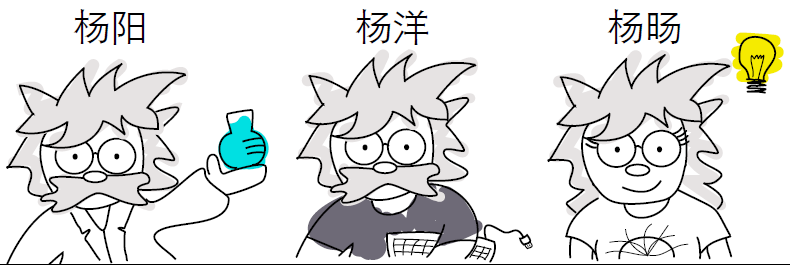
\includegraphics[width=\textwidth]{./figures/homonym.png}
\end{figure}

\end{frame}


% Entity Resolution ==============================================================


\begin{frame}{Author Disambiguation as Entity Resolution Problem}

\begin{figure}
   \centering
   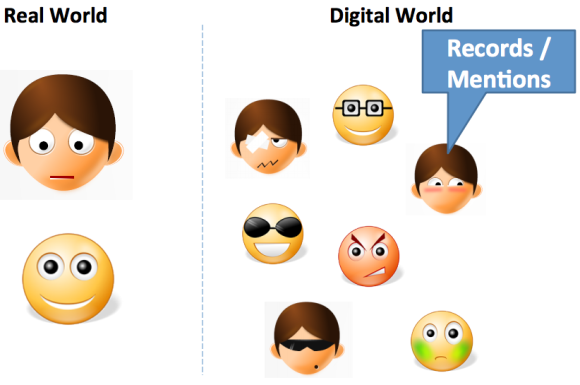
\includegraphics[width=\textwidth]{./figures/entity_resolution.png}
\end{figure}

Image source: datacommunitydc.org
\end{frame}


% Table of content==========
%\begin{frame}{Overview}
%\tableofcontents[pausesections]
%\end{frame}
%==========

% Definitions ====================================================================


\section{Definitions}

\subsection{From publications to signatures}

\begin{frame} {Definitions}

\begin{figure}
   \centering
   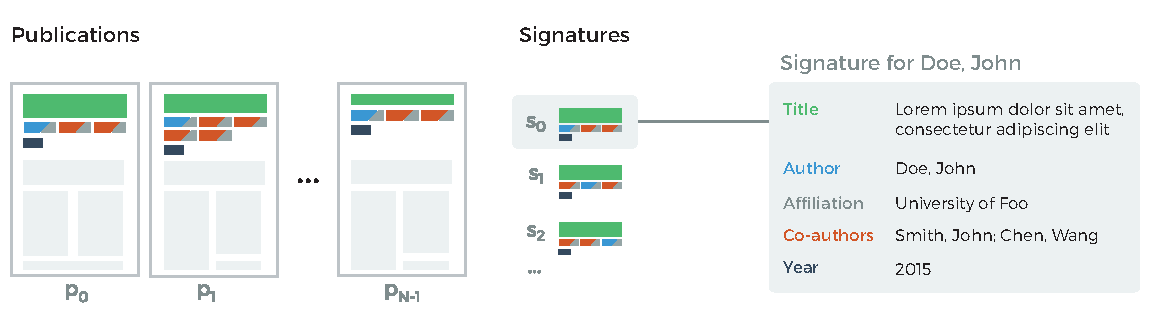
\includegraphics[width=\textwidth]{./figures/fig-pub-to-signature.pdf}
\end{figure}

\end{frame}


% Problem statement ==================================================================

% IMPORTANT Explain what the boxes represent.

\begin{frame}{Problem to Solve}
For each author, group together all his publications, and only those.

\begin{block}{Inspirehep.net is a digital library contains}
\begin{itemize}
\item  Over 1M publication forming more than 10M signatures
\item  1.2M signatures are claimed by:\\[1em]
\begin{itemize}
\item Authors themselves (similar to Google Scholar). \\[1em]
\item Universal identifiers (ORCiD) . \\[1em]
\item Professional curators . \\[1em]
\end{itemize}
\end{itemize}
\end{block}
\end{frame}


%=================================================
\begin{frame}{Problem Formulation}

\tikzstyle{block} = [rectangle, draw, text width=10em, text centered, rounded corners, minimum height=2em]
\tikzstyle{line} = [draw, -latex']
\tikzstyle{cloud} = []

\begin{center}
\begin{tikzpicture}[node distance = 2cm, auto]
    % Place nodes
    \node [block] (clustering) {Author disambiguation};
    \node [cloud, above of=clustering] (input1) {$\{s_1, s_2, ..., s_N\}$};
    \node [cloud, below of=clustering] (output) {$\{ \underbrace{\{ s_1, s_3, s_4 \}}_{\text{author 1}}, \underbrace{\{ s_2, s_5\}}_{\text{author 2}}, ... \}$};
    % Draw edges
    \path [line] (input1) -- (clustering);
    \path [line] (clustering) -- (output);
\end{tikzpicture}
\end{center}
\end{frame}

% Learning ====================================================================


\section{Linkage function}

\begin{frame}{Learning from data}

\begin{itemize}
\item Manual disambiguation is {\color{red} long and difficult}, even for experienced curators.\\[2em]
\item Couldn't we {\color{blue} automatically find a set of rules} to disambiguate two signatures?

$$\varphi(s_1, s_2) = \begin{cases}
    0 & \text{if $s_1$ and $s_2$ belong to the same author},\\
    1 & \text{otherwise}.
  \end{cases}$$

\item This is a machine learning task called {\color{red}supervised learning}.
\end{itemize}

\end{frame}


% Ethnicity Features ========================================================

\subsection{Ethnicity Features}
\begin{frame}{Ethnicity Features}

\begin{figure}
   \centering
   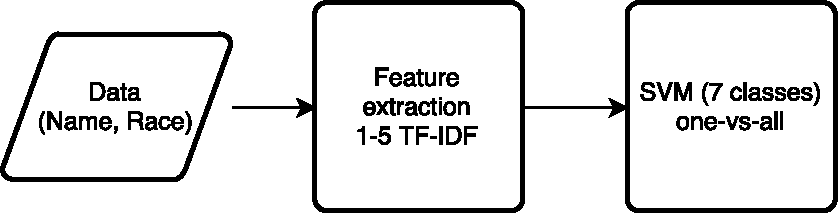
\includegraphics[width=.7\textwidth]{./figures/ethnicity.pdf}
\end{figure}
 From (IPUMS-USA) we extracted:
\begin{itemize}

\item White: 20M
\item Black: 3M
\item American Indian or Alaska Native: 150K
\item Chinese: 50K
\item Japanese: 50K
\item Other Asian or Pacific Islander: 30K
\item Other race: 1K
\end{itemize}


\end{frame}

% Pair-wise Features Extraction ========================================================

\subsection{Feature engineering}
\begin{frame}{Pair-wise Features Extraction}

\begin{figure}
   \centering
   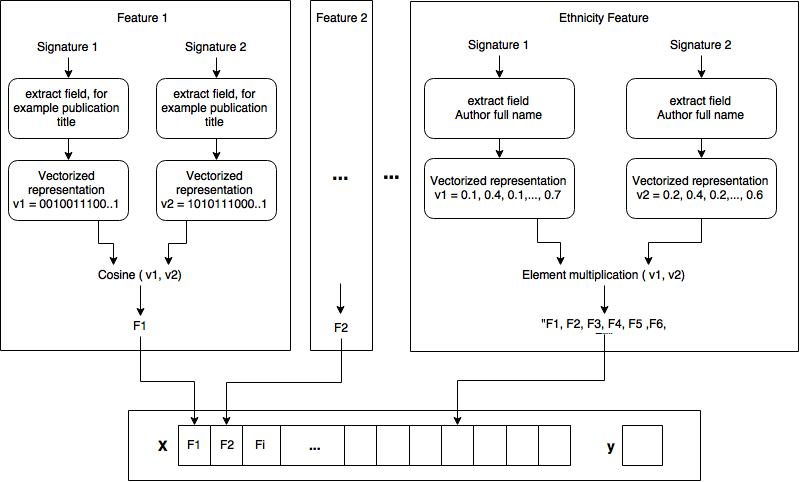
\includegraphics[width=\textwidth]{./figures/pairwise_features.png}
\end{figure}

\end{frame}

% Features ====================================================================

\begin{frame}{Features set}
\begin{table}
\label{table:features}
\centering
{\small
\begin{tabular}{|l|l|}
  \hline
  \textbf{Feature} & \textbf{Combination operator}\\
  \hline
  \hline
  Full name & Cosine similarity of $(2,4)$-TF-IDF\\
  Given names & Cosine similarity of $(2,4)$-TF-IDF\\
  First given name & Jaro-Winkler distance\\
  Second given name & Jaro-Winkler distance\\
  Given name initial & Equality\\
  Affiliation & Cosine similarity of $(2,4)$-TF-IDF\\
  Co-authors & Cosine similarity of TF-IDF\\
  Title & Cosine similarity of $(2,4)$-TF-IDF\\
  Journal & Cosine similarity of $(2,4)$-TF-IDF\\
  Abstract & Cosine similarity of TF-IDF\\
  Keywords & Cosine similarity of TF-IDF\\
  Collaborations & Cosine similarity of TF-IDF\\
  References & Cosine similarity of TF-IDF\\
  Subject & Cosine similarity of TF-IDF\\
  Year difference & Absolute difference\\
  \hline
  Any ethnicity feature & Product of probabilities estimated by SVM\\
  \hline
\end{tabular}}
\end{table}
\end{frame}




% Feature Importances by Recursive Elimination ========================================================

\begin{frame}{Feature Importances by Recursive Elimination}

\begin{figure}
   \centering
   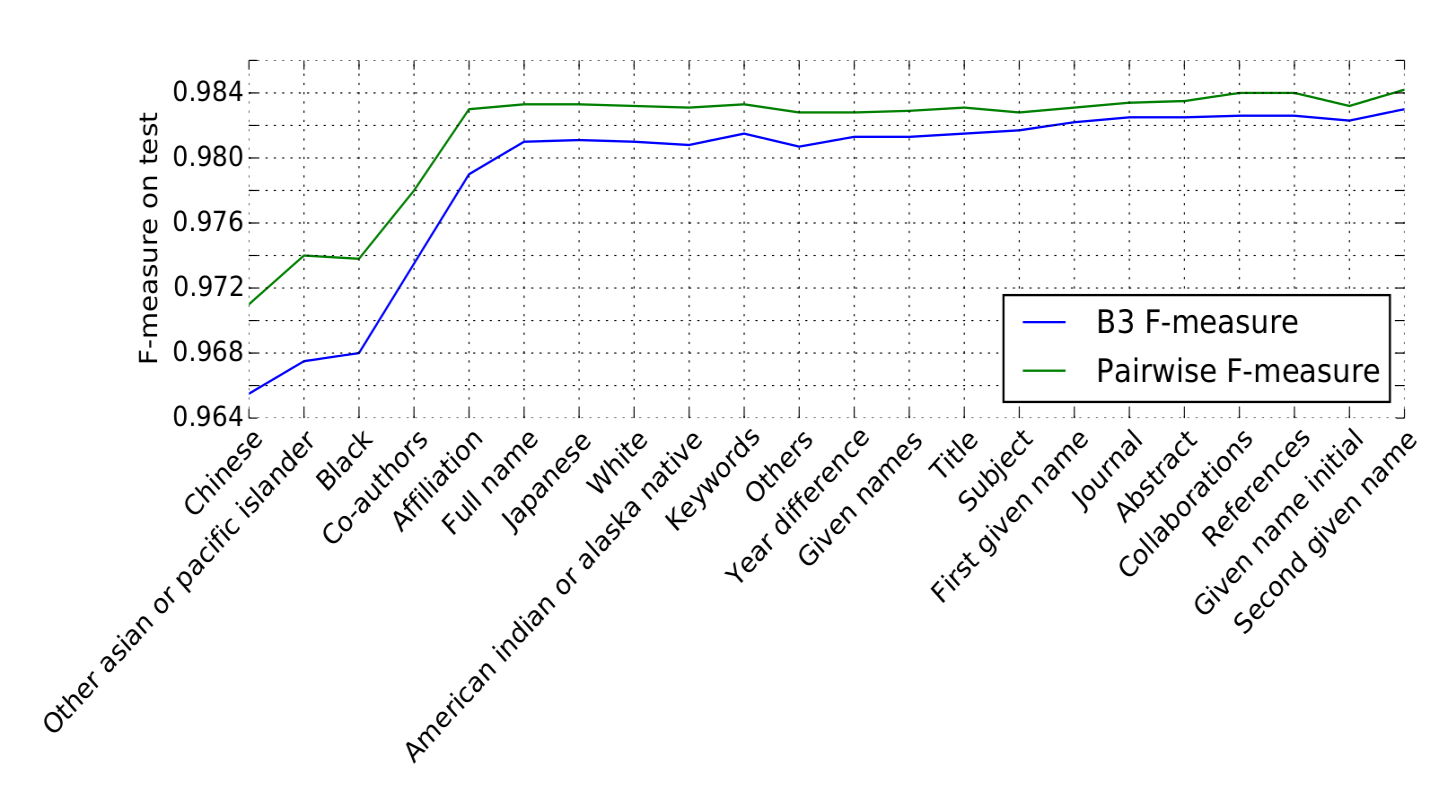
\includegraphics[width=\textwidth]{./figures/fig-rfe.png}
\end{figure}

\end{frame}


\section{Clustering}

\begin{frame}{Disambiguation as a clustering problem}

\tikzstyle{block} = [rectangle, draw, text width=10em, text centered, rounded corners, minimum height=2em]
\tikzstyle{line} = [draw, -latex']
\tikzstyle{cloud} = []

\begin{center}
\begin{tikzpicture}[node distance = 2cm, auto]
    % Place nodes
    \node [block] (clustering) {Author disambiguation};
    \node [cloud, above of=clustering] (input1) {$\{s_1, s_2, ..., s_N\}$};
    \node [cloud, below of=clustering] (output) {$\{ \underbrace{\{ s_1, s_3, s_4 \}}_{\text{author 1}}, \underbrace{\{ s_2, s_5\}}_{\text{author 2}}, ... \}$};
    % Draw edges
    \path [line] (input1) -- (clustering);
    \path [line] (clustering) -- (output);
\end{tikzpicture}
\end{center}
\end{frame}


% Hierarchical clustering =====================================================

\begin{frame}{Hierarchical Clustering}

\begin{columns}[T]

\begin{column}{0.33\textwidth}
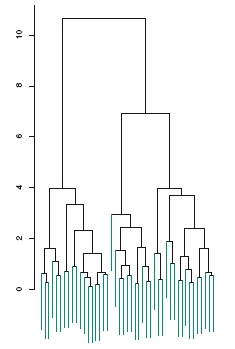
\includegraphics[scale=0.75]{./figures/hierarchy.png}
\end{column}
\begin{column}{0.66\textwidth}
\begin{itemize}
\item General family of clustering algorithms that {\color{blue}build nested clusters by merging them successively}.\\[2em]

\item This hierarchy of clusters is represented as a tree (or dendrogram).\\[2em]

\item The root of the tree is the unique cluster that gathers all the samples, the leaves being the clusters with only one sample.
\end{itemize}
\end{column}

\end{columns}

\end{frame}


% Implementation issues =====================================================

\section{Clustering issues}

\begin{frame}{Clustering Issues}

\begin{itemize}
\item The complexity of hierarchical clustering is {\color{red} $O(N^2)$}. For $N=10^7$ signatures, this is impractical.

{\it {\color{blue}Solution:}} partitioning into blocks all signatures with the same last name + first initial, then cluster each of these blocks.\\[2em]

\item How do you set the {\color{red} cut-off threshold}?

{\it {\color{blue}Solution:}} using training data (e.g., claimed signatures), pick the threshold that locally maximizes some criterion.
\end{itemize}

\end{frame}


\begin{frame} {General Pipeline}


\begin{figure}
   \centering
   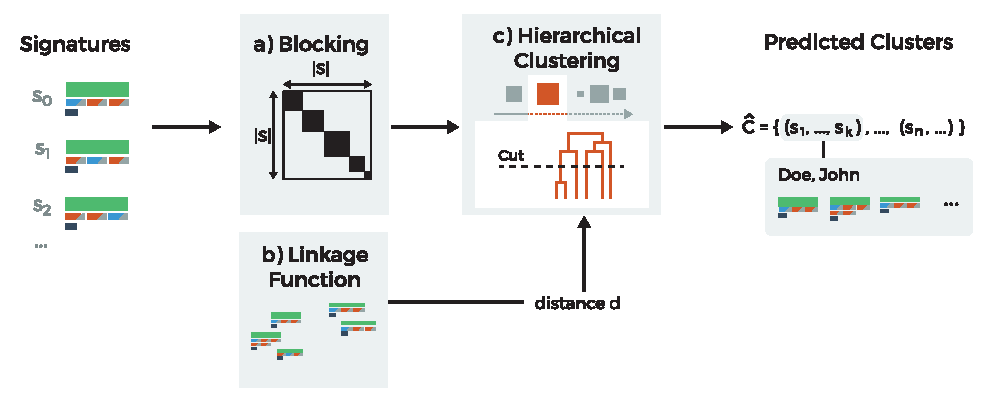
\includegraphics[width=\textwidth]{./figures/fig-workflow.pdf}
\end{figure}

\end{frame}

% Partitioning into Blocks =====================================================

% No reason to describe the dataset here


\subsection{Blocking}

\begin{frame} {Solving Issue 1: Partitioning into Blocks}


\begin{figure}
   \centering
   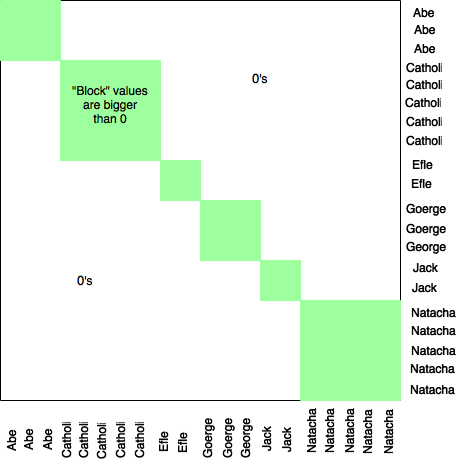
\includegraphics[width=0.7\textwidth]{./figures/blocking.png}
\end{figure}

% What we need to do in order to reduce the complexity of the clustering step is to
% partition all the signatures into blocks and then run the clustering algorithm for all
% the blocks. This step in the previous works was called blocking and thus we will stick to
% this name. It's important to say here what a good blocking algorithm should do. Firstly,
% should minimize the number of pairs of signatures that belong to the same author but
% after blocking step can not be clustered together, and sum of squares of the sizes of
% produced blocks, so basically the computational cost of the clustering. 

% It is important to say here that if the size of the blocks is on average around 100, maybe
% sometimes  1000 signatures, than effectively the algorithm becomes linear.

% However, those two objectives that I mentioned are hard to achieve together.

% The simpliest strategy, that was commonly used in the past is what we call "Surname
% and first initial". It works like this: we take all the signatures with the same
% surname and the same first initial, and we group them together. 
% (describe image)

% There are some limitations of this method.

%\end{itemize}

%\end{column}


\end{frame}

% Cases =====================================================


\begin{frame} {Cases}

Analysis of data showed that author can have multiple names in few cases:

\begin {itemize}
 \item "Mueller, R." and "Muller, R."

  \item "Martinez Torres, A." and "Torres, A. Martinez"

  \item "Smith-Jones, A." and "Smith, A."

  \item "Smith, Jack" and "Smith, A. J."

  \item An authors surname changed (e.g., due to marriage).

\end {itemize}

% We decided to do some analysis on our training set. We took the pairs that belong to the
% same author but are represented by different names and we noticed that 1). it happens
% often and 2). there are some patterns. We manually decided what the patterns are, and
% here they are:

\end{frame}

% Blocking Strategies =====================================================


\begin{frame} {Solution}


\begin{figure}
   \centering
   \includegraphics[width=0.9\textwidth]{./figures/Blocking.png}
\end{figure}

% Name the phonetic algorithms (Soundex, NYSIIS, Metaphone)

%This algorithm effectively solves paragraphs 1-3 from the previous page without %introducing
%many errors. As the blocks were still too large, we split them over the first given name
%initital.

\end{frame}


% Cutting Strategy =====================================================


\subsection{Cut-off strategies}

\begin{frame} {Solving Issue 2: Threshold Cut-off Strategy}

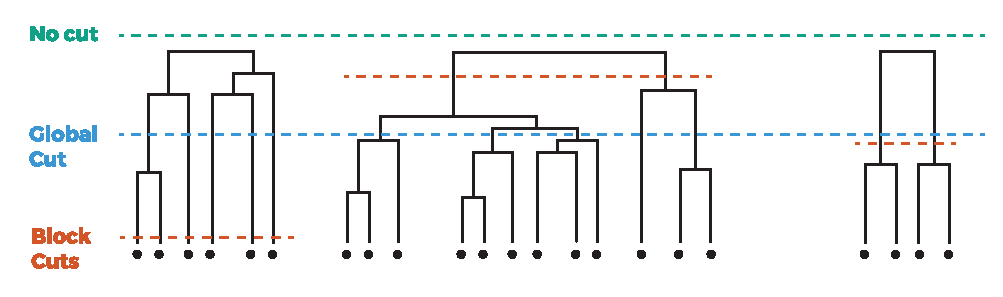
\includegraphics[width=\textwidth]{./figures/fig-cuts.pdf}

% The second problem that Hussein mentioned is that we need to decide how to cut the
% dendograms that are produced. So, first of all notice that if we have a blocking phase,
% than we have one dendogram for every block. We decided to try 3 different approaches.


% Simply by iterating over all possible

% Blocks cut (new concept)

\end{frame}


% Evaluation =====================================================================

\section{Evaluation}

\begin{frame}{Evaluation}

{\it Protocol:} Use the {\color{blue} claimed signatures} (about 1M) to form {\color{blue} ground truth clusters}. Keep 10\% as a training set to find model parameters, and 90\% as a test set for evaluation.

\begin{align}
\text{$B^3$ Precision} &= \mathbb{E}_s \{ \frac{|\hat{C}(s) \cap C(s)|}{|\hat{C}(s)|}  \} \\
\text{$B^3$ Recall} &= \mathbb{E}_s \{ \frac{|\hat{C}(s) \cap C(s)|}{|C(s)|}  \} \\
\text{$B^3$ F-score} &= \frac{2 \times \text{Precision} \times \text{Recall}}{\text{Precision} + \text{Recall}}
\end{align}

where $C(s)$ (resp., $\hat{C}(s)$) is the true (resp., predicted) set of signatures to which $s$ belongs.


% As our task is clustering, we need to have a measure for comparing the scores.
% There are two popular approaches. //paired and b3

% We chose b3 as ... (balancing...)

% give number for simple strategy (all same names baseline 0.5, all same block baseline 1.0)
\end{frame}

% Results =====================================================================


\section{Results}

\begin{frame}{Results 1 of 2}

% What is baseline

% Mention recall improvement

% Ensemble because better for heterogenous data, can easily find non-linear dependencies
% (and they are in the dataset).

\begin{table}
%\caption{Average precision, recall and f-measure scores on test folds. Underlined row %corresponds to the state-of-the-art choices.}
\centering
\begin{tabular}{|l|c c c |}
  \hline
                       & \multicolumn{3}{|c|}{\textbf{$B^{3}$}}\\
  \textbf{Description} & $Prec.$ & $Recall$ & $F1$ \\
  \hline
  \hline
Baseline & 0.9024 & 0.9828 & 0.9409  \\
\hline
\underline{Blocking = Surname \& First Initial} & 0.9901 & 0.9760 & 0.9830  \\
Blocking = Double metaphone & 0.9856 & 0.9827 & 0.9841  \\
Blocking = NYSIIS & 0.9875 & 0.9826 & \textbf{0.9850}   \\
Blocking = Soundex & 0.9886 & 0.9745 & 0.9815  \\
\hline
\underline{Classifier = Gradient Boosting Classifier} & 0.9901 & 0.9760 & 0.9830   \\
Classifier = Random Forests & 0.9909 & 0.9783 & \textbf{0.9846}  \\
Classifier = Linear Regression & 0.9749 & 0.9584 & 0.9666 \\
\hline
Training pairs = Non-blocked, uniform & 0.9793 & 0.9630 & 0.9711   \\
Training pairs = Blocked, uniform & 0.9854 & 0.9720 & 0.9786   \\
\underline{Training pairs = Blocked, balanced} & 0.9901 & 0.9760 & \textbf{0.9830}  \\
\hline

\end{tabular}
\end{table}

\end{frame}

% Results =====================================================================

% One can say it's not much, but if you take a look into the number of the problems solved,
% then ..

\begin{frame}{Results 2 of 2}

\begin{table}
%\caption{Average precision, recall and f-measure scores on test folds. Underlined row %corresponds to the state-of-the-art choices.}
\centering
\begin{tabular}{|l|c c c |}
  \hline
                       & \multicolumn{3}{|c|}{\textbf{$B^{3}$}}\\
  \textbf{Description} & $Prec.$ & $Recall$ & $F1$ \\
  \hline
  \hline
Baseline & 0.9024 & 0.9828 & 0.9409  \\
\hline
\underline{Clustering = Average linkage} & 0.9901 & 0.9760 & \textbf{0.9830}  \\
Clustering = Single linkage & 0.9741 & 0.9603 & 0.9671  \\
Clustering = Complete linkage & 0.9862 & 0.9709 & 0.9785   \\
\hline
No cut (baseline) & 0.9024 & 0.9828 & 0.9409   \\
Global cut & 0.9892 & 0.9737 & 0.9814   \\
\underline{Block cut} & 0.9901 & 0.9760 & \textbf{0.9830} \\
\hline
\textbf{Combined best settings} & 0.9888 & 0.9848 & \textbf{0.9868}  \\
Best settings without ethnicity features & 0.9862 & 0.9819 & 0.9841 \\
\hline

\end{tabular}
\end{table}

\end{frame}

% Results =====================================================================

\begin{frame}{Summary Results}

\begin{table}
    \centering
    \begin{tabular}{| l c |}
    \hline
        \textit{Method} & \textit{$B^3 \text{F-score}$}  \\
    \hline
    \hline
    Full name & 0.8183 \\
    Last name + First initial & 0.9409 \\
    \hline
    Our model & {\color{blue} 0.9868} \\
    \hline
    \end{tabular}
\end{table}

\end{frame}


% Performance ================================================================

\begin{frame}{Implementation}

The solution is currently being used by the INSPIRE and INVENIO projects at CERN. \\[1em]

% mention that we are aware of two companies that use our solution

Execution time: $20$ hours for 10M signatures, on a $16$ cores machine with $32$GB of RAM. 

{\color{red} But}, even only few minutes for incremental disambiguation! \\[1em]

% explain

% why did you release?

% mention the work from the previous day, you can install library with pip (python package
% manager)

Our solution is open-source\footnote{\url{github.com/inspirehep/beard}} and we released the
dataset\footnote{\url{github.com/glouppe/paper-author-disambiguation/data}}.

% use by other companies

\end{frame}

\begin{frame}{Conclusions}

\begin{itemize}
\item Semi-supervised approach on the biggest dataset ever used for author disambiguation.
\item Novel blocking technique based on phonetization.
\item Showing the significancy of inferred name ethnicity.
\item Showing the importance of balancing the training set.
\end{itemize}

\end{frame}

% Future Work ================================================================

\begin{frame}{Future Work}

\begin{itemize}

\item Error analysis.\\[1em]

\item Build or find more comprehensive name-ethnicity dataset. \\[1em]

\item Explore author embedding approaches as a blocking strategy.\\[1em]

\item Build phonetic algorithm tailored to the disambiguation task. \\[1em]

\item Archive and utilize user's feedback to enhance the model. \\[1em]

\item Try our disambiguation solution for other tasks. 

\end{itemize}

\end{frame}


\end{document}
